\documentclass[10pt,a4paper]{ltjsarticle}       % LuaTeX を使う
\usepackage[luatex]{graphicx}             % LuaTeX 用, draft がついているときは図の代わりに同じ大きさの枠ができる
\usepackage{here}                               % 図表の位置を強制して出力
\usepackage{afterpage}                          % 残っている図を貼り付ける(\afterpage{\clearpage})
\usepackage[subrefformat=parens]{subcaption}    % サブキャプション(図1(a) とか)
\usepackage{setspace}                           % 行間制御
\usepackage{ulem}                               % 下線や取り消し線など
\usepackage{booktabs}                           % きれいな表(\toprule \midrule \bottomrule)
\usepackage{multirow}                           % 表で行結合
\usepackage{multicol}                           % 表で列結合
\usepackage{hhline}                             % 表で 2 重線
\usepackage[table]{xcolor}                      % カラー
\usepackage{tikz}                               % 図描画用
\usepackage[framemethod=tikz]{mdframed}         % 文章を囲むとき用
\usepackage[version=3]{mhchem}                  % 化学式
\usepackage{siunitx}                            % 単位
\usepackage{comment}                            % コメント
\setcounter{tocdepth}{3}                        % 目次に subsubsection まで表示
\usepackage{listings}
\lstdefinelanguage{Julia}%
  {morekeywords={abstract,break,case,catch,const,continue,do,else,elseif,%
      end,export,false,for,function,immutable,import,importall,if,in,%
      macro,module,otherwise,quote,return,switch,true,try,type,typealias,%
      using,while},%
   sensitive=true,%
   alsoother={\$},%
   morecomment=[l]\#,%
   morecomment=[n]{\#=}{=\#},%
   morestring=[s]{"}{"},%
   morestring=[m]{'}{'},%
}[keywords,comments,strings]%

\lstset{%
    language         = Julia,
    basicstyle       = \ttfamily,
    keywordstyle     = \bfseries\color{blue},
    stringstyle      = \color{magenta},
    commentstyle     = \color{ForestGreen},
    showstringspaces = false,
}
%\lstset{
%    frame=single,
%    basicstyle=\small\ttfamily,
%    tabsize=4,
%    language=python,
%    keywordstyle=\color{red},
%    stringstyle=\color{blue}
%}

% -----ヘッダ・フッタの設定-----
\usepackage{fancyhdr}
\usepackage{lastpage}
\pagestyle{fancy}
\lhead{}                                 % 左ヘッダ
\chead{}                                 % 中央ヘッダ
\rhead{}                                 % 右ヘッダ
\lfoot{}                                 % 左フッタ
\cfoot{\thepage~/~\pageref{LastPage}}    % 中央フッタ
\rfoot{}                                 % 右フッタ
\renewcommand{\headrulewidth}{0pt}       % ヘッダの罫線を消す
% -----余白の設定-----
% これをアンコメントするとページ番号が中央からずれるから今は使わない.
% \usepackage[left=19.05mm,right=19.05mm,top=25.40mm,bottom=25.40mm]{geometry}
% -----フォントの設定-----
% https://ja.osdn.net/projects/luatex-ja/wiki/LuaTeX-ja%E3%81%AE%E4%BD%BF%E3%81%84%E6%96%B9
% http://myfuturesightforpast.blogspot.jp/2013/12/tex-gyre.html など
\usepackage[no-math]{fontspec}
\usepackage{amsmath,amssymb}    % 高度な数式用
\usepackage{mathrsfs}           % 花文字用
% times ベース -> txfonts
% palatino ベース -> pxfonts
\usepackage{txfonts}
\usepackage{bm}                 % 斜体太字ベクトル
% Avant Garde -> TeX Gyre Adventor
% Bookman Old Style -> TeX Gyre Bonum
% Zapf Chancery -> TeX Gyre Chorus
% Courier -> TeX Gyre Cursor
% Helvetica -> TeX Gyre Heros
% Helvetica Narrow -> TeX Gyre Heros Cn
% Palatino -> TeX Gyre Pagella
% New Century Schoolbook -> TeX Gyre Schola
% Times -> TeX Gyre Termes
\setmainfont[Ligatures=TeX]{TeXGyreTermes}
\setsansfont[Ligatures=TeX]{TeXGyreHeros}
\setmonofont[Scale=MatchLowercase]{TeXGyreCursor}
\usepackage[match,deluxe,expert,bold]{luatexja-fontspec}
\setmainjfont[BoldFont=IPAexGothic]{IPAexMincho}
\setsansjfont{IPAexGothic}
\usepackage{luatexja-otf}
% -----PDF ハイパーリンク,ブックマーク,URL の設定-----
% オプション(\hypersetup{})は https://texwiki.texjp.org/?hyperref 参照
\usepackage{url}
% -----ソースコードの設定-----
% オプション(\lstset{})は http://tug.ctan.org/tex-archive/macros/latex/contrib/listings/listings.pdf 参照
% 使うときは
% \begin{lstlisting}[language=aaaa,caption=bbbb,label=List:cccc]
% hogehoge
% \end{lstlisting}
\usepackage{listings}
\lstset{%
  basicstyle=\ttfamily\small,%
  frame=single,%
  frameround=ffff,%
  numbers=left,%
  stepnumber=1,%
  numbersep=1\zw,%
  breaklines=true,%
  tabsize=4,%
  captionpos=t,%
  commentstyle=\itshape}
% -----図表等の reference の設定-----
% 表示文字列を日本語化
\renewcommand{\figurename}{図}
\renewcommand{\tablename}{表}
\renewcommand{\lstlistingname}{リスト}
\renewcommand{\abstractname}{概要}
% 図番号等を"<章番号>.<図番号>"
% lstlisting に関しては https://tex.stackexchange.com/questions/134418/numbering-of-listings 参照
\renewcommand{\thefigure}{\thesection.\arabic{figure}}
\renewcommand{\thetable}{\thesection.\arabic{table}}
\AtBeginDocument{\renewcommand{\thelstlisting}{\thesection.\arabic{lstlisting}}}
\renewcommand{\theequation}{\thesection.\arabic{equation}}
% 節が進むごとに図番号等をリセット
% http://d.hatena.ne.jp/gp98/20090919/1253367749 参照
\makeatletter
\@addtoreset{figure}{section}
\@addtoreset{table}{section}
\@addtoreset{lstlisting}{section}
\@addtoreset{equation}{section}
\makeatother
% \ref{} の簡単化
\newcommand*{\refSec}[1]{\ref{#1}~章}
\newcommand*{\refSsec}[1]{\ref{#1}~節}
\newcommand*{\refSssec}[1]{\ref{#1}~項}
\newcommand*{\refFig}[1]{\figurename~\ref{#1}}
\newcommand*{\refTab}[1]{\tablename~\ref{#1}}
\newcommand*{\refList}[1]{\lstlistingname~\ref{#1}}
\newcommand*{\refEq}[1]{式~(\ref{#1})}
% -----数式中便利な定義-----
% https://www.library.osaka-u.ac.jp/doc/TA_LaTeX2.pdf
% https://en.wikibooks.org/wiki/LaTeX/Mathematics など
\newcommand{\e}{\mathrm{e}}                     % ネイピア数
\newcommand{\imagi}{\mathrm{i}}                 % 虚数単位(i)
\newcommand{\imagj}{\mathrm{j}}                 % 虚数単位(j)
\newcommand{\vDel}{\varDelta}                   % デルタ大文字
\newcommand{\veps}{\varepsilon}                 % イプシロン小文字
\newcommand*{\paren}[1]{\left( #1 \right)}      % () を中身の大きさに合わせる
\newcommand*{\curly}[1]{\left\{ #1 \right\}}    % {} を中身の大きさに合わせる
\newcommand*{\bracket}[1]{\left[ #1 \right]}    % [] を中身の大きさに合わせる
\renewcommand{\Re}{\operatorname{Re}}           % 実部
\renewcommand{\Im}{\operatorname{Im}}           % 虚部
\newcommand*\sfrac[2]{{}^{#1}\!/_{#2}}          % xfrac パッケージの \sfrac{}{} の代わり
\renewcommand*\vec[1]{\mathbf{#1}}              % 矢印ベクトルは使わないので上書き.太字立体.
\newcommand{\argmax}{\mathop{\rm arg~max}\limits}
\newcommand{\argmin}{\mathop{\rm arg~min}\limits}

\title{知的システム論第10回レポート}
\author{37186305\\航空宇宙工学専攻修士一年\\荒居秀尚}
\begin{document}
\maketitle
\section{宿題}
Julia 1.0.0によりMNIST datasetのうちtestデータを次元削減・クラスタリング・可視化した。実装は以下の通りである。
\begin{lstlisting}
using LinearAlgebra
using Flux.Data.MNIST
using Plots

function PCA(X, m)
    d = size(X)[1]
    n = size(X)[2]
    C = zeros((d, d))
    for i in 1:n
        C += X[:, i] * X[:, i]'
    end

    eigs = eigen(C)
    T = zeros((m, d))
    last = d - m + 1
    for (i, j) in enumerate(d:-1:last)
        vec = eigs.vectors[:, j]
        T[i, :] = vec'
    end
    T * X
end

function converged(array, tol)
    mean = 0.0
    for i in 1:length(array)
        mean += sum(array[i].^2)
    end
    mean < tol
end


function calc_center(X)
    n = size(X)[2]
    ret = [0, 0]
    for i in 1:n
        ret += X[:, i]
    end
    ret ./ n
end


function KMeans(X, c, tol=1e-5)
    d = size(X)[1]
    n = size(X)[2]
    centers = [rand(2,1) for _ in 1:c]
    before = [[100, 100] for _ in 1:c]
    cpreds = zeros(n)
    while !converged(before - centers, tol)
        for i in 1:n
            norms = [sum((X[:, i] - center).^2) for center in centers]
            label = argmin(norms)
            cpreds[i] = label
        end
        before = centers
        idxs = [findall(cpreds .== i) for i in 1:c]
        centers = [ifelse(X[idx] != [], calc_center(X[:, idx]), before[i]) for (i, idx) in enumerate(idxs)]
    end
    return centers, cpreds
end

imgs = MNIST.images(:test)
X = hcat(float.(vec.(imgs))...)
X_pca = PCA(X, 2)
centers, cpreds = KMeans(X_pca, 10)
p = plot(xlabel="x", ylabel="y", title="Compressed image of MNIST")
colors = [:green, :blue, :red, :yellow, :pink, :black, :gold, :silver, :brown, :purple]
for (i, c) in enumerate(colors)
    idx = findall(cpreds .== i)
    scatter!(X_pca[1, idx], X_pca[2, idx], color=c, label=string(i))
end
png("scatter")

labels = MNIST.labels(:test)
p = plot(xlabel="x", ylabel="y", title="Compressed image of MNIST with true label")
colors = [:green, :blue, :red, :yellow, :pink, :black, :gold, :silver, :brown, :purple]
for (i, c) in enumerate(colors)
    idx = findall(labels .== i)
    scatter!(X_pca[1, idx], X_pca[2, idx], color=c, label=string(i))
end
png("scatter_true")
\end{lstlisting}

この結果が以下のようになった。
\begin{figure}[htbp]
\begin{center}
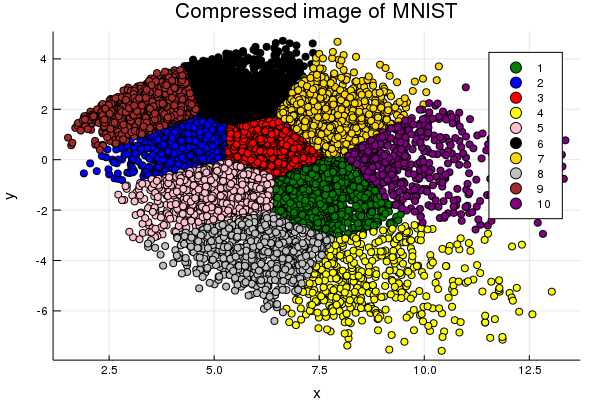
\includegraphics[clip, scale=0.6]{scatter.png}
\caption{KMeansによるクラスタリング}
\end{center}
\end{figure}

\begin{figure}[htbp]
\begin{center}
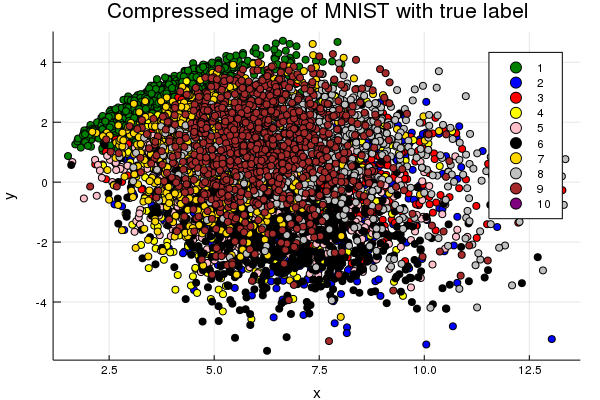
\includegraphics[clip, scale=0.6]{scatter_true.png}
\caption{正解ラベルごとに色分けした図}
\end{center}
\end{figure}

この二枚の図を見比べるとそもそも784次元空間のものを2次元に射影して考えることに無理があるとわかる。また、KMeansの境界付近が直線になっており、ボロノイ境界が見えることがわかる。
\end{document}